%%%%%%%%%%%%%%%%%%%%%%%%%%%%%%%%%%%%%%%%%
% Beamer Presentation
% LaTeX Template
% Version 1.0 (10/11/12)
%
% This template has been downloaded from:
% http://www.LaTeXTemplates.com
%
% License:
% CC BY-NC-SA 3.0 (http://creativecommons.org/licenses/by-nc-sa/3.0/)
%
%%%%%%%%%%%%%%%%%%%%%%%%%%%%%%%%%%%%%%%%%

%----------------------------------------------------------------------------------------
%	PACKAGES AND THEMES
%----------------------------------------------------------------------------------------

\documentclass{beamer}

\mode<presentation> {

% The Beamer class comes with a number of default slide themes
% which change the colors and layouts of slides. Below this is a list
% of all the themes, uncomment each in turn to see what they look like.

%\usetheme{default}
%\usetheme{AnnArbor}
%\usetheme{Antibes}
%\usetheme{Bergen}
%\usetheme{Berkeley}
%\usetheme{Berlin}
%\usetheme{Boadilla}
%\usetheme{CambridgeUS}
%\usetheme{Copenhagen}
%\usetheme{Darmstadt}
%\usetheme{Dresden}
%\usetheme{Frankfurt}
%\usetheme{Goettingen}
%\usetheme{Hannover}
%\usetheme{Ilmenau}
%\usetheme{JuanLesPins}
%\usetheme{Luebeck}
\usetheme{Madrid}
%\usetheme{Malmoe}
%\usetheme{Marburg}
%\usetheme{Montpellier}
%\usetheme{PaloAlto}
%\usetheme{Pittsburgh}
%\usetheme{Rochester}
%\usetheme{Singapore}
%\usetheme{Szeged}
%\usetheme{Warsaw}

% As well as themes, the Beamer class has a number of color themes
% for any slide theme. Uncomment each of these in turn to see how it
% changes the colors of your current slide theme.

%\usecolortheme{albatross}
%\usecolortheme{beaver}
%\usecolortheme{beetle}
%\usecolortheme{crane}
%\usecolortheme{dolphin}
%\usecolortheme{dove}
%\usecolortheme{fly}
%\usecolortheme{lily}
%\usecolortheme{orchid}
%\usecolortheme{rose}
%\usecolortheme{seagull}
%\usecolortheme{seahorse}
%\usecolortheme{whale}
%\usecolortheme{wolverine}

%\setbeamertemplate{footline} % To remove the footer line in all slides uncomment this line
%\setbeamertemplate{footline}[page number] % To replace the footer line in all slides with a simple slide count uncomment this line

%\setbeamertemplate{navigation symbols}{} % To remove the navigation symbols from the bottom of all slides uncomment this line
}

\usepackage{listings}
\usepackage{graphicx} % Allows including images
\usepackage{booktabs} % Allows the use of \toprule, \midrule and \bottomrule in tables
\usepackage[T1]{fontenc}
\usepackage[utf8]{inputenc}
\newcommand{\light}[1]{\textcolor{lightgray}{#1}}

%----------------------------------------------------------------------------------------
%	TITLE PAGE
%----------------------------------------------------------------------------------------

\title[Kvalifikacioni Ispit]{Kvalifikacioni Ispit} % The short title appears at the bottom of every slide, the full title is only on the title page

\author{Bogdan Vukobratović} % Your name
\institute[FTN] % Your institution as it will appear on the bottom of every slide, may be shorthand to save space
{
Fakultet Tehničkih Nauka \\ % Your institution for the title page
\medskip
\textit{bogdan.vukobratovic@gmail.com} % Your email address
}
\date{09.06.2016.} % Date, can be changed to a custom date

\begin{document}

\begin{frame}
\titlepage % Print the title page as the first slide
\end{frame}

%\begin{frame}
%\frametitle{Overview} % Table of contents slide, comment this block out to remove it
%\tableofcontents % Throughout your presentation, if you choose to use \section{} and \subsection{} commands, these will automatically be printed on this slide as an overview of your presentation
%\end{frame}

%----------------------------------------------------------------------------------------
%	PRESENTATION SLIDES
%----------------------------------------------------------------------------------------

%------------------------------------------------
% \section{} % Sections can be created in order to organize your presentation into discrete blocks, all sections and subsections are automatically printed in the table of contents as an overview of the talk
%------------------------------------------------

% \subsection{Subsection Example} % A subsection can be created just before a set of slides with a common theme to further break down your presentation into chunks

\begin{frame}
\frametitle{Predlog naslova doktorske disertacije}
\huge{\centerline{“Hardverska akceleracija algoritama}}
\huge{\centerline{za formiranje celih stabala odluke}}
\huge{\centerline{i njihovih ansambala”}}
\end{frame}

%------------------------------------------------

\begin{frame}
\frametitle{Cilj istraživanja - Motivacija}
\begin{itemize}
\setlength{\itemsep}{\fill}
\item Cilj istraživanja - razvoj algoritama za indukciju celih stabala
odluke i njihova efikasna implementacija u “embedded” sistemima.
\item Algoritmi za indukciju celih stabala odluke proizvode kompaktnija
stabla:
\begin{itemize}
\item Okamova oštrica: jednostavnije = bolje
\vspace{1em}
\item Jednostavnija stabla $\implies$ manje hardverskih resursa
\end{itemize}
\end{itemize}
\end{frame}

%------------------------------------------------

\begin{frame}
\frametitle{Cilj istraživanja}
\begin{enumerate}
\setlength{\itemsep}{\fill}
\item EFTI - Novi evolutivni algoritam za indukciju celih neortogonalnih stabala
odluke, koji ne zahteva populaciju
\item EFTIP - Hardverska arhitektura za akceleraciju EFTI algoritma
\item EEFTI - Novi evolutivni algoritam za indukciju ansambala neortogonalnih celih
stabala odluke na bazi EFTI algoritma
\item DTEEP - Hardverska arhitektura za akceleraciju EEFTI algoritma
\end{enumerate}
\end{frame}

%------------------------------------------------

\begin{frame}[fragile]
\frametitle{Stabla odluke}
\begin{figure}
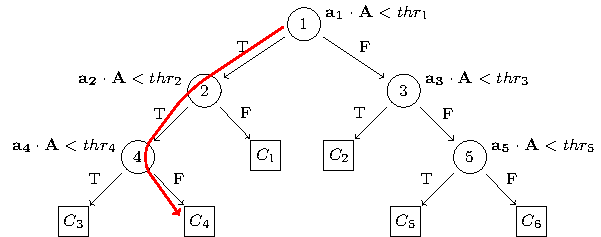
\includegraphics[width=0.7\linewidth]{oblique_dt_traversal.pdf}
\end{figure}
\begin{itemize}
\setlength{\itemsep}{\fill}
\item Intuitivan model, visok stepen imunosti na šum, podjednako dobar kako za numeričke tako i za kategoričke atribute, mogućnost rada sa redundantnim ili nedostajućim atributima itd.
\item Pronalaženje optimalnog testa u čvoru je NP-težak problem $\implies$ upotrebljavaju se heuristike
\item Dva generalna pristupa indukciji: inkrementalni (čvor-po-čvor, ``greedy'') i celo stablo odjednom
\end{itemize}
\end{frame}

%------------------------------------------------

\begin{frame}
\frametitle{Plan rada - EFTI 1/3}
\begin{enumerate}
\setlength{\itemsep}{\fill}
\item EFTI - Novi evolutivni algoritam za indukciju celih neortogonalnih stabala
odluke, koji ne zahteva populaciju
\item\light{EFTIP - Hardverska arhitektura za akceleraciju EFTI algoritma}
\item\light{EEFTI - Novi evolutivni algoritam za indukciju ansambala neortogonalnih celih
stabala odluke na bazi EFTI algoritma}
\item\light{DTEEP - Hardverska arhitektura za akceleraciju EEFTI algoritma}
\end{enumerate}
\end{frame}

%------------------------------------------------

\begin{frame}
\frametitle{Plan rada - EFTI 2/3}
\begin{itemize}
\setlength{\itemsep}{\fill}
\item Evoluira samo jednu jedinku
\item Algoritam je evolutivan, te podrazumeva:
\begin{itemize}
\setlength{\itemsep}{\fill}
\item Mutaciju - nasumičnu izmenu jedinke u nadi za unapređenjem fitnesa.
\begin{itemize}
\item Mutacija koeficijenata testova u čvorovima
\item Oduzimanje/dodavanje čvorova
\end{itemize}
\item Evaluaciju fitnesa - meru kvaliteta jedinke na osnovu parametara od interesa: tačnost, veličina, prisutnost svih klasa problema u listovima, čistoća listova, balansiranost, itd.
\item Selekciju - odlučivanje o prihvatanju mutirane jedinke
\begin{itemize}
\item Ako je ostvaren napredak u fitnesu
\item Nasumično, iako je jedinka slabijeg fitnesa $\implies$ beg iz lokalnog optimuma
\end{itemize}
\end{itemize}
\end{itemize}
\end{frame}

%------------------------------------------------

\begin{frame}[fragile]
\frametitle{Plan rada - EFTI 3/3}
\small\begin{lstlisting}[language=Python]
def efti(train_set):
    initialize(dt)
    best_fit = fitness_eval(dt, train_set)

    for iter in range(max_iter):
        dt_mut = mutate(dt)
        cur_fit = fitness_eval(dt_mut, train_set)

        if (cur_fit > best_fit) or (random() < p_escape):
            best_fit = cur_fit
            dt = dt_mut

    return dt
\end{lstlisting}
\end{frame}

%------------------------------------------------

\begin{frame}
\frametitle{Plan rada - EFTIP 1/3}
\begin{enumerate}
\setlength{\itemsep}{\fill}
\item\light{EFTI - Novi evolutivni algoritam za indukciju celih neortogonalnih stabala
odluke, koji ne zahteva populaciju}
\item EFTIP - Hardverska arhitektura za akceleraciju EFTI algoritma
\item\light{EEFTI - Novi evolutivni algoritam za indukciju ansambala neortogonalnih celih
stabala odluke na bazi EFTI algoritma}
\item\light{DTEEP - Hardverska arhitektura za akceleraciju EEFTI algoritma}
\end{enumerate}
\end{frame}

%------------------------------------------------

\begin{frame}
\frametitle{Plan rada - EFTIP 2/3}
\begin{itemize}
\setlength{\itemsep}{\fill}
\item Kompleksnost računanja fitnesa (\(N_{I}\) - broj instanci u trening setu, \emph{n} -
broj atributa i \emph{D} - prosečna dužina puta instance kroz stablo )\\
\vspace{1em}
\centerline{$T(fitness\_eval) = O(N_{I}\cdot D\cdot n)$}
\item HW/SW kodizajn pristup akceleraciji EFTI-ja
\begin{itemize}
\item Računanje fitnesa $\implies$ hardver
\item Mutacija i selekcija $\implies$ softver
\end{itemize}
\end{itemize}
\end{frame}

%------------------------------------------------

\begin{frame}[fragile]
\frametitle{Plan rada - EFTIP 3/3}
\begin{figure}
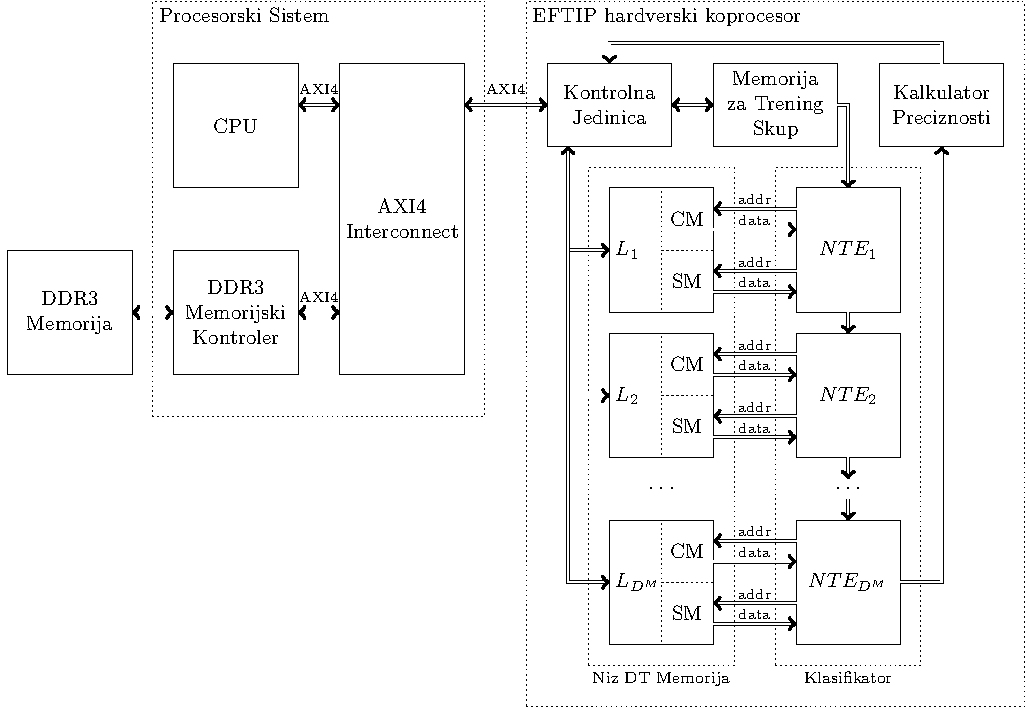
\includegraphics[width=0.9\linewidth]{eftip_architecture.pdf}
\end{figure}
\end{frame}

%------------------------------------------------

\begin{frame}
\frametitle{Plan rada - EEFTI 1/3}
\begin{enumerate}
\setlength{\itemsep}{\fill}
\item\light{EFTI - Novi evolutivni algoritam za indukciju celih neortogonalnih stabala
odluke, koji ne zahteva populaciju}
\item\light{EFTIP - Hardverska arhitektura za akceleraciju EFTI algoritma}
\item EEFTI - Novi evolutivni algoritam za indukciju ansambala neortogonalnih celih
stabala odluke na bazi EFTI algoritma
\item\light{DTEEP - Hardverska arhitektura za akceleraciju EEFTI algoritma}
\end{enumerate}
\end{frame}

%------------------------------------------------

\begin{frame}
\frametitle{Plan rada - EEFTI 2/3}
\begin{itemize}
\setlength{\itemsep}{\fill}
\item ``Bagging'' algoritam za indukciju ansambala
\begin{itemize}
\item Podela trening skupa na podskupove $\implies$ svaki podskup za indukciju jednog člana
\end{itemize}
\vspace{1em}
\vspace{1em}
\item Potpuni ``decoupling'' između procesa indukcije članova $\implies$ idealno za paralelizaciju
\end{itemize}
\end{frame}

%------------------------------------------------

\begin{frame}[fragile]
\frametitle{Plan rada - EEFTI 3/3}
\small\begin{lstlisting}[language=Python]
def efti(train_set, ensemble_size):
    task_train_sets = divide_train_set(train_set, ensemble_size)

    res = []
    initialize_result_array(res, ensemble_size)

    for t, r in zip(task_train_sets, res):
        create_task(efti_task, t, r)

    wait_for_all_tasks()

    return res
\end{lstlisting}
\end{frame}

%------------------------------------------------

\begin{frame}
\frametitle{Plan rada - DTEEP 1/3}
\begin{enumerate}
\setlength{\itemsep}{\fill}
\item\light{EFTI - Novi evolutivni algoritam za indukciju celih neortogonalnih stabala
odluke, koji ne zahteva populaciju}
\item\light{EFTIP - Hardverska arhitektura za akceleraciju EFTI algoritma}
\item\light{EEFTI - Novi evolutivni algoritam za indukciju ansambala neortogonalnih celih
stabala odluke na bazi EFTI algoritma}
\item DTEEP - Hardverska arhitektura za akceleraciju EEFTI algoritma
\end{enumerate}
\end{frame}

%------------------------------------------------

\begin{frame}
\frametitle{Plan rada - DTEEP 2/3}
\begin{itemize}
\setlength{\itemsep}{\fill}
\item Kompleksnost računanja fitnesa (\(N_{I}\) - broj instanci u trening setu, \emph{n} -
broj atributa i \emph{D} - prosečna dužina puta instance kroz stablo )\\
\vspace{1em}
\centerline{$T(fitness\_eval) = O(N_{I}\cdot D\cdot n)$}
\item HW/SW kodizajn pristup akceleraciji EFTI-ja
\begin{itemize}
\item Računanje fitnesa $\implies$ hardver
\item Mutacija i selekcija $\implies$ softver
\end{itemize}
\end{itemize}
\end{frame}

%------------------------------------------------

\begin{frame}[fragile]
\frametitle{Plan rada - DTEEP 3/3}
\begin{figure}
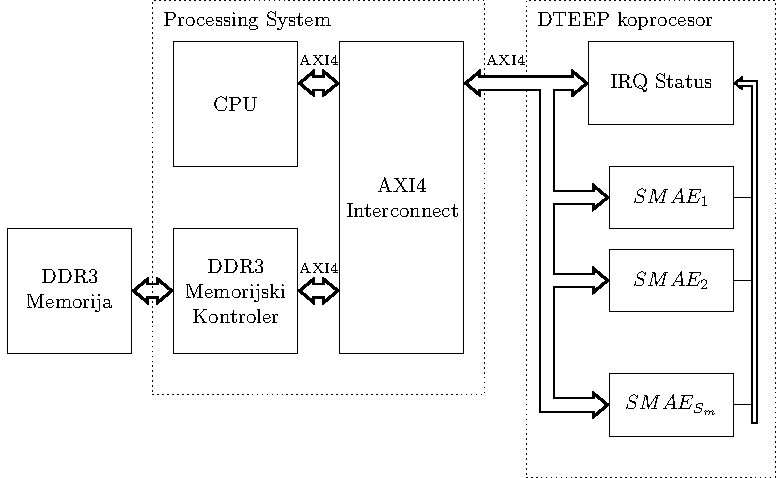
\includegraphics[width=0.9\linewidth]{dteep_architecture.pdf}
\end{figure}
\end{frame}

%------------------------------------------------

\begin{frame}
\frametitle{Metode}
\begin{itemize}
\setlength{\itemsep}{\fill}
\item Poređenje C implementacije EFTI algoritma po brzini i tačnosti sa ostalim standardnim algoritmima: OC1, CART, HBDT, GaTree, GALE itd.
\item \emph{UCI} baza standardnih ulaznih problema
\item Poređenje HW/SW kodizajnova na osnovu EFTIP i DTEEP koprocesora sa čistim softverskim implementacijama EFTI i EEFTI algoritama
\end{itemize}
\end{frame}

%------------------------------------------------

\begin{frame}
\Huge{\centerline{Hvala na pažnji!}}
\end{frame}

%----------------------------------------------------------------------------------------

\end{document}
